\chapter{Application: Style Based Tonemapping}
\label{chp:b5}

\section{Problem Definition}

The existence of numerous tone mapping operators that are available paved the way for many studies have are conducted for selecting the best one [40]. However, tone mapping can be conducted for different purposes, and rendering the resulting images to follow a consistent style can be one of them. For example, in a movie production process, making all frames consistently tone mapped, regardless of the content of the frames, can be a desired operation to impart a certain look and feel to the viewers. Although obtaining different renderings from tone mapping operators is partly achievable by using different tone mapping parameters, some tone mapping operators have none[ref!] or few parameters[ref!] while others[ref!] have too many. Besides, even though one set of parameters are found for a certain image to depict a certain style of rendering, the same set of parameters would not yield with the same look when applied to other images. Akyüz et al. [2] proposes a style based tone mapping operator that aims to consistently tone map different HDR images with the defined style.

\section{Method}
Style based tone mapping [2] consists of two consecutive phases, namely \emph{calibration} and \emph{operation}. Calibration is the phase where the user defines a style and operation is the phase that the user given HDR image is tone mapped with the predefined style in the calibration phase. Figure \ref{fig:calibration_operation} shows the style based tone mapping algorithm steps and these steps are explained in the next sections.

\begin{figure}
\begin{center}
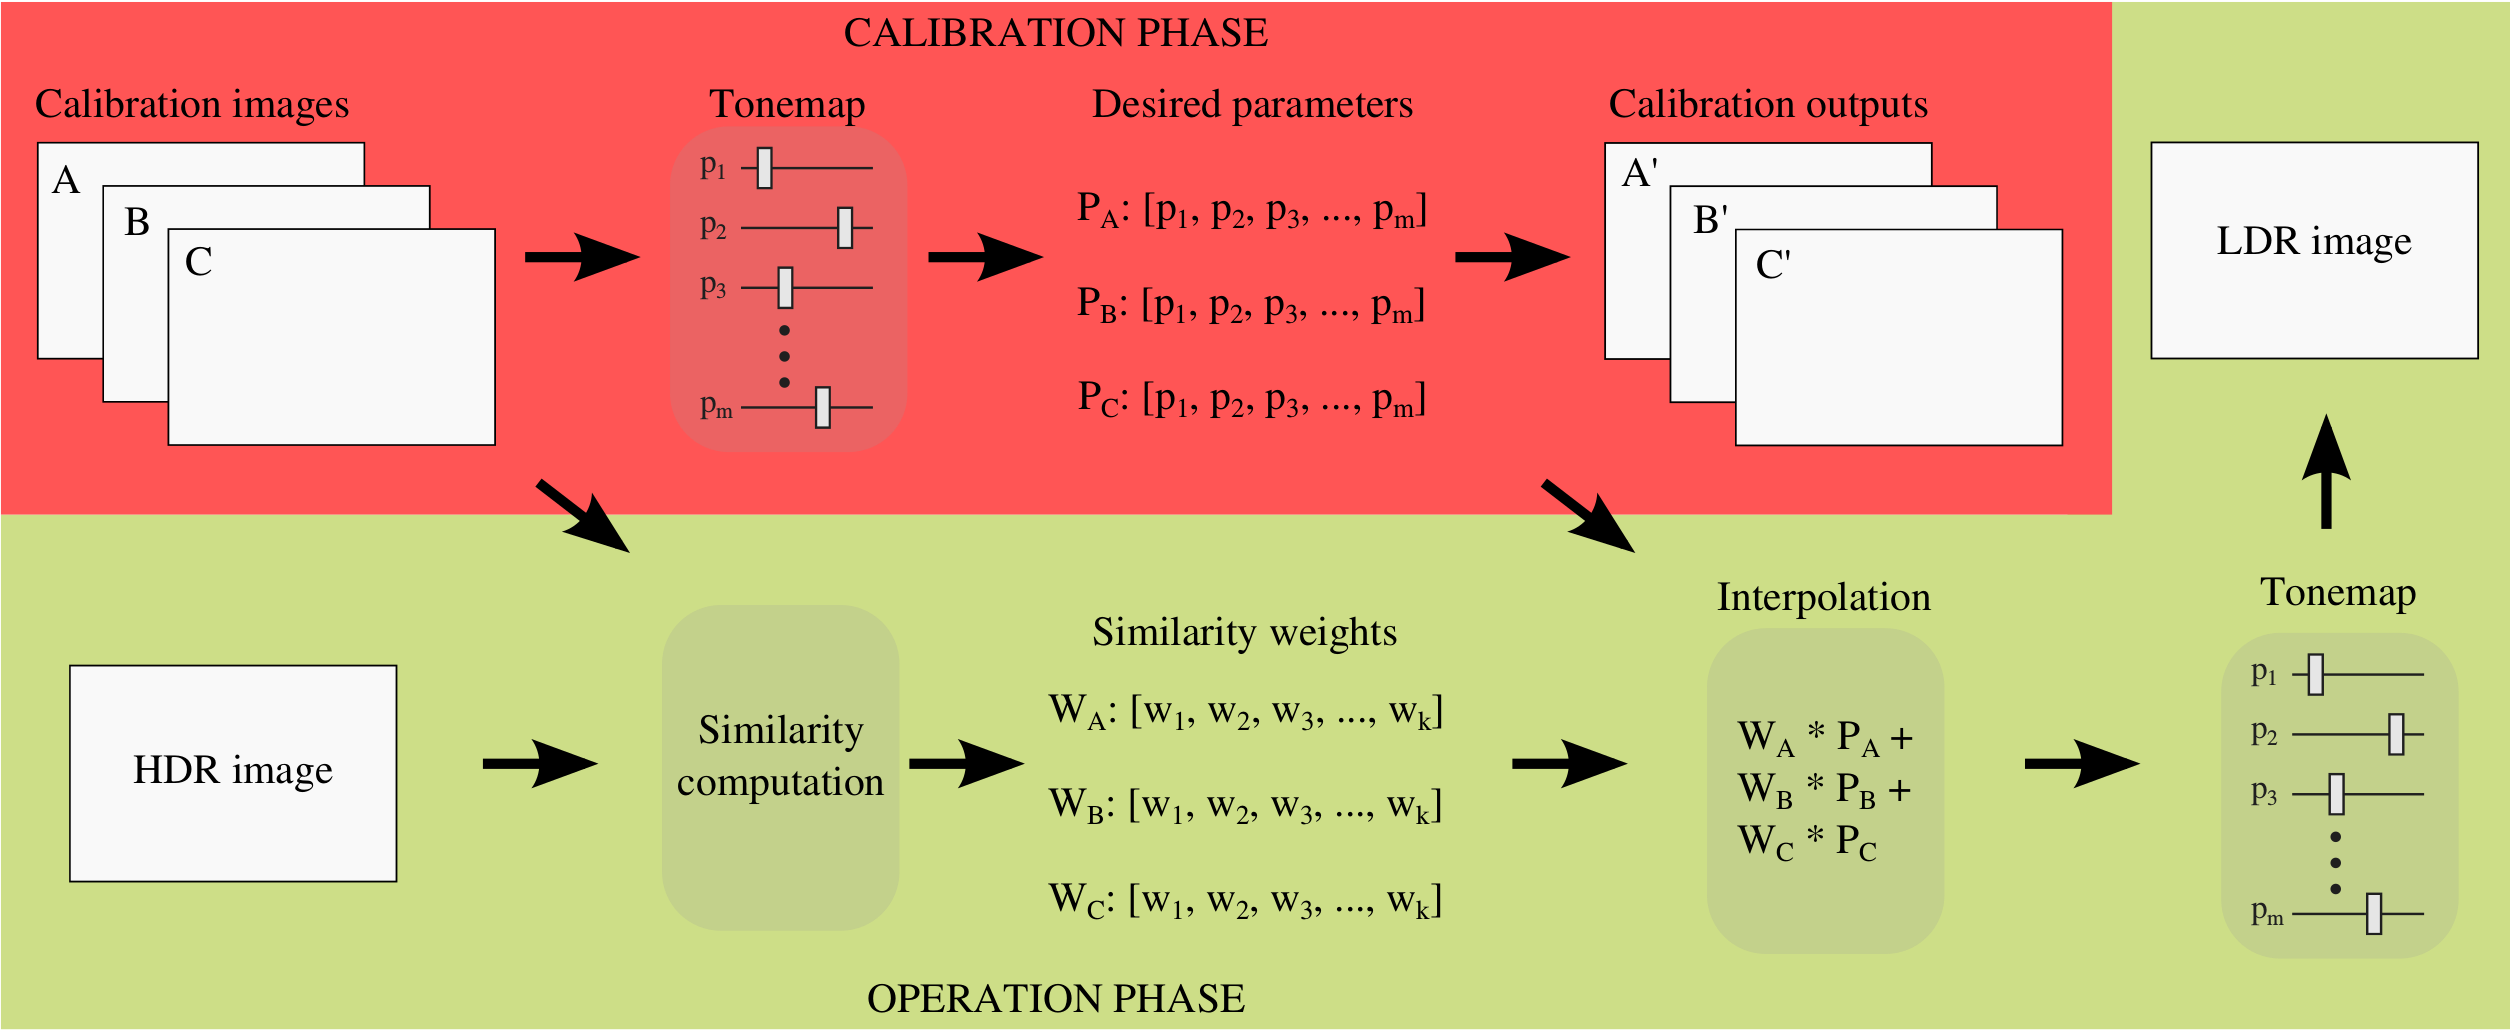
\includegraphics[width=\textwidth]{figures/chapter5/temp_calibration_operation.png}
\caption{Calibration and operation phases of style based tone mapping}
\label{fig:calibration_operation}
\end{center}
\end{figure}

\subsection{Calibration}
In the calibration phase, first the user is asked to pick a name for the new style to be created, and then the user is required to tone map a fixed set of calibration images. Assigning a name to the style would be helpful for the user to stay consistent with the style while tone mapping the calibration images and once the style is created and saved, will be helpful to have many predefined styles in preset library and reuse them. 

Calibration images should be representative enough for different environments that has different characteristics and distinctive from each other to keep the number of the calibration images low. The number of calibration images directly affects the duration of the calibration phase, so although more calibration images would represent different environments better, in order not to overwhelm the user, the number of calibration images is chosen in a way that the user can finish the calibration phase in a reasonable time.

Calibration images are selected in a semi automatic way. First, all images are taken from Fairchild's HDR image dataset [!ref] and then converted a feature space and using k-means algorithm divided into different clusters. After clusters are obtained, one calibration image is hand-selected from each cluster, yielding 6 calibration images in total, which are shown in Figure \ref{fig:calibration_images}.

\begin{figure}
\begin{center}
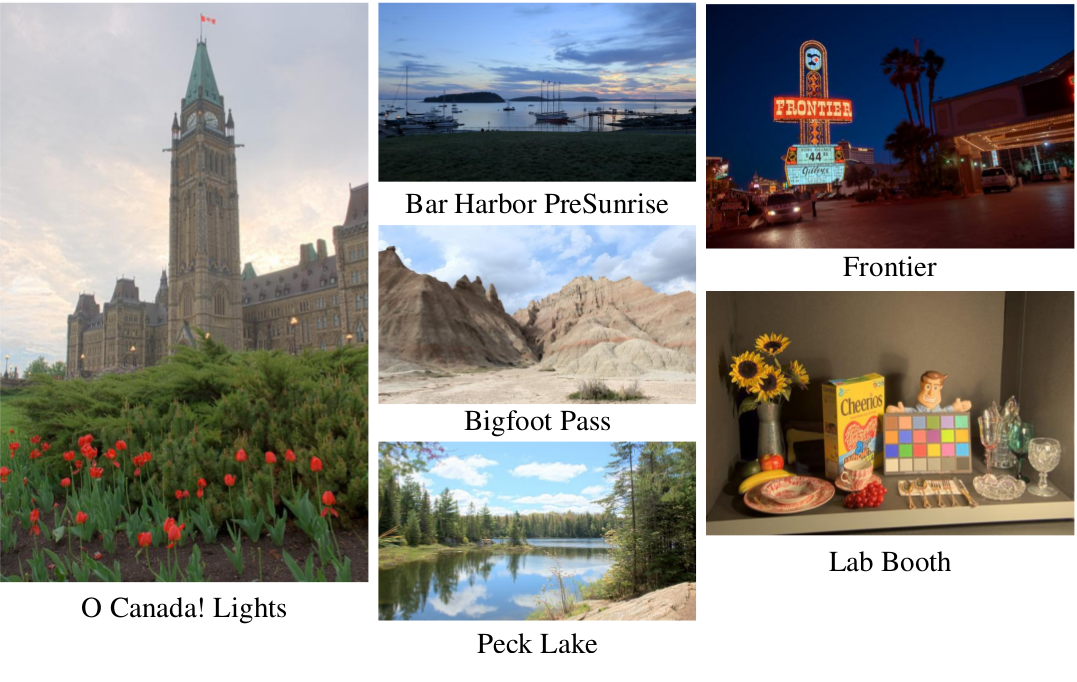
\includegraphics[width=\textwidth]{figures/chapter5/temp_calibration_images.png}
\caption{Calibration images
%paper
}
\label{fig:calibration_images}
\end{center}
\end{figure}

After naming the style, the user is presented with the tone mapping interface and required to tone map the calibration images one after another with the desired style. The manual tone mapping procedure is basically adjusting tone mapping parameters given in Table \ref{tab:tonemap_parameters}.

\begin{table}[h!]
\caption{Tone mapping parameters for style-based tone mapping}
\label{tab:tonemap_parameters}
\centering
\begin{tabular}{|c|c|}
\hline 
Brightness ($b$) & Prct. mapped to half-max intensity \\
Contrast ($c$) & Slope of the tone curve at $b$ \\
Black point ($bp$) & Prct. clamped to min intensity \\
White point ($wp$) & Prct. clamped to max intensity \\
Color saturation ($c$) & Saturation control exponent \\
\hline
Small detail strength ($\lambda_s$) & UM factor for small details \\
Medium detail strength ($\lambda_m$) & UM factor for medium details \\
Large detail strength ($\lambda_l$) & UM factor for large details \\
\hline
\end{tabular}
\end{table}

The tone mapping operator is a modified version of Generic TMO[ref!]. Generic TMO models many existing tone mapping operator, both local and global with a tone curve followed by a spatial modulation function. It is note in [ref!] that same set of parameters yields very different results for different images. Style based tone mapping uses Generic TMO with the following modifications.

Tone mapping parameters of Generic TMO are replaced with their percentile counterparts in order to make the algorithm less image dependent. For example, the parameter \emph{Brightness} in style based tone mapping with the value 50 would correspond to the median brightness value of the HDR image in Generic TMO's \emph{b} parameter. Likewise, for the parameter \emph{White point}, the value 95 would mean 5\% of the brightest pixels will be burned out. As one may imagine, representing the tone mapping parameters as percentiles is not sufficient to achieve the same effect on different images. In order to achieve this, style based tone mapping uses parameter interpolation to use \emph{similar} parameters to \emph{similar} images as described in Section \ref{sec:operation}. 

The second modification to Generic TMO belongs to spatial modulation. In [!ref], a linear combination of band-pass filters as spatial modulation function. These filters are from modified Cortex transform and applied after global tone curve modulation. On the other hand, in style based tone mapping, local modulation is applied in multiple scales and then global operation is performed. This has the benefit of adjusting detail level before the HDR compression and gives better results. 

For detail modulation several approaches has been tested, unsharp masking (UM), bileteral filtering [!ref] and gradient reversal removed BF[!ref]. While BF-based filters results with less halo, they are computationally expensive, unlike UM, which is prone to halos but computationally efficient. Besides, UM is shown to be improve sharpness and local contrast in an earlier study [!ref]. It is decided to use UM even though it may introduce halos. For some cases, halos may be also introduced by the user in order to create an unrealistic style.

The detail modulation is achieved by first creating three low-pass images in the logarithmic domain for $small$, $medium$ and $large$ details.

\begin{align}
L'_{\sigma_s} = g _{\sigma_s} * L', \\
L'_{\sigma_m} = g _{\sigma_m} * L', \\
L'_{\sigma_l} = g _{\sigma_l} * L', 
\end{align}

where $L' = log L$ and $g_\sigma$ are 2D Gaussian filters are different scales. $\sigma_s$, $\sigma_m$, and $\sigma_l$ are set to 0.0625\%, 0.3125\% and 0.625\% of the minimum image dimension respectively. Then these low pass images are used to enhance different scales with the chosen detail factor parameters $\lambda$.

\begin{equation}
    L_{sm} = e^{L' + \lambda_s(L' - L'_{\sigma_s}) + \lambda_m(L'_{\sigma_s} - L'_{\sigma_m}) + \lambda_l(L'_{\sigma_m} - L'_{\sigma_l})}
\end{equation}

$L_{sm}$, spatially modulated luminance image, then fitted to the tone curve as in [ref!]. 

\begin{equation}
    TC(L_{sm}) = 
    \begin{cases}
    0 \text{  if  $L_{sm}' \leq b - d_l$ } \\
    \frac{1}{2}c {{L_{sm}' - b}\over{1 - a_l(L_{sm}'-b)}} + \frac{1}{2} \text{ if $b - d_l < L_{sm}' \leq b $ } \\ 
    \frac{1}{2}c {{L_{sm}' - b}\over{1 + a_h(L_{sm}'-b)}} + \frac{1}{2} \text{ if $b < L_{sm}' \geq b + d_h$} \\ 
    1 \text{ if  $L_{sm}' > b + d_h$}
    \end{cases}
\end{equation}

where $L_{sm}'$ is the logarithm of the spatially modulated luminance $c$ is the contrast, and parameters $b$, $d_l$ and $d_h$ are the absolute values of the user given parameters in percentiles for brightness, black point and white point respectively. Parameters $a_h$ and $a_l$ are contrast compression for light and dark areas computed from [!ref].

\begin{equation}
    a_l = {{c . d_l-1} \over {d_l}} \text{ and } a_h = {{c . d_h-1} \over {d_h}}
\end{equation}

In Figure \ref{fig:calibration_phase}, the user interface that allows the user to define a style for tone mapping during the calibration phase is shown. The tone mapping parameters can be easily adjusted with the sliders and the calibration image will be tone mapped and shown to the user in real time. The luminance histograms of log HDR and LDR images are also shown to aid the user and show the effect of the changes. After all of the calibration images are tone mapped, the style parameters are saved and the calibration phase finishes.

\begin{sidewaysfigure}
\begin{center}
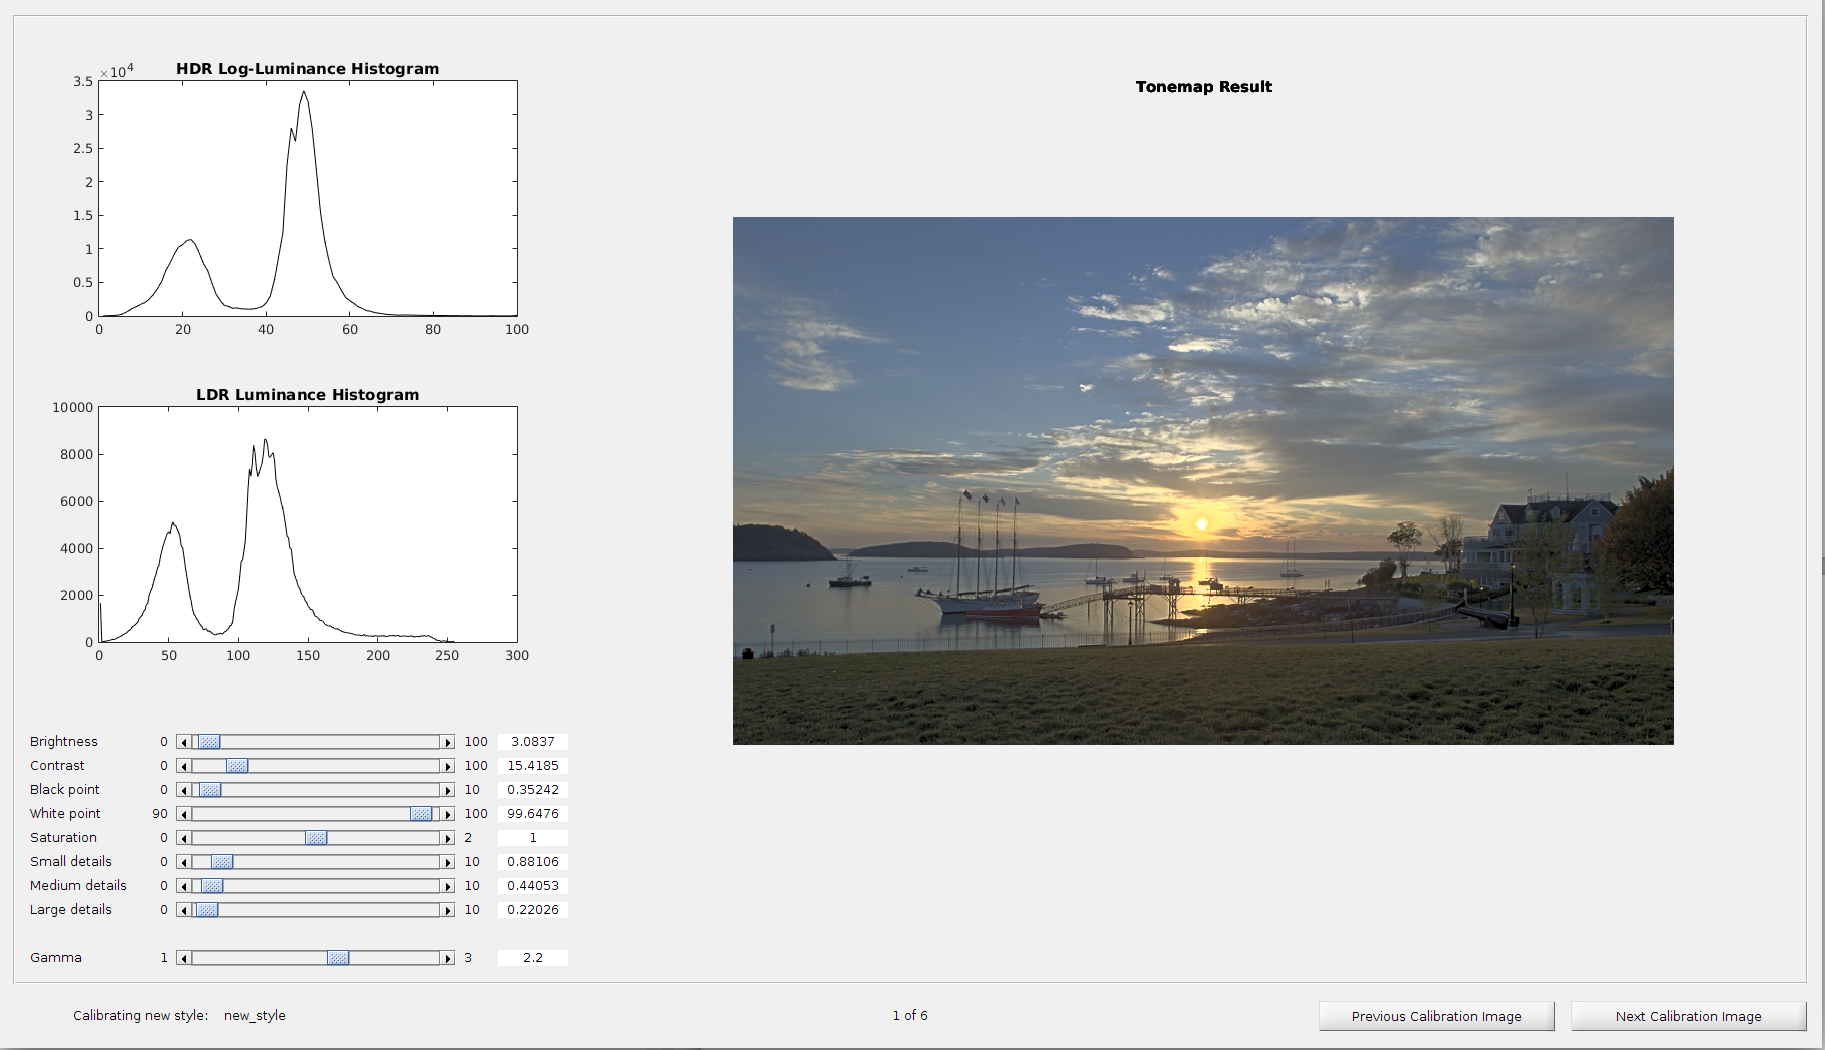
\includegraphics[width=\textwidth]{figures/chapter5/ui_screenshot.png}
\caption{User interface for calibration phase}
\label{fig:calibration_phase}
\end{center}
\end{sidewaysfigure}

\subsection{Operation}
\label{sec:operation}
In the operation phase, user selects a style from preset library that has been created in the calibration phase. Given a new HDR image to be tone mapped with the selected style, the tone mapping parameters \emph{t} (given in Table \ref{tab:tonemap_parameters}) must be determined based on calibration image tone mapping parameters \emph{$t_i$}. Style based tone mapping approaches this problem as image similarity problem. If two images are similar according to a similarity metric, their tone mapping parameters should be also similar. After the distances between input image and the calibration images, the tone mapping parameters are calculated as inverse distance transform [!ref]:

\begin{equation}
\label{eq:inv_distance_transform}
    \mathbf{t} = {{\sum _{i=1} ^{N} {1 \over {d(\mathbf{f}, \mathbf{f_i})}} \mathbf{t_i}} \over {\sum _{i=1} ^{N} {1 \over {d(\mathbf{f}, \mathbf{f_i})}}}}
\end{equation}

Here, $\mathbf{f}$ is the feature vector of the current input image and $\mathbf{f_i}$ the feature vector for the calibration image $i$ and $\mathbf{t}$ its computed tone mapping parameters. Lastly, the function $d$ calculates the similarity between two feature vectors.

In [2], images are represented with HSV histograms [ref] and histograms of gradients [ref] to capture colorimetric and structural properties of the images. HDR images varies highly on pixel values and it is hard to compare them directly. To overcome this, images are tone mapped to the interval $[0,1]$:

\begin{equation}
    L_{out} = {{L_{in}} \over {1 + L_{in}}}, 
\end{equation}

and color channels are transformed with:

\begin{equation}
    \mathbf{C_{out}} = {{\mathbf{C_{in}}}\over{L_{in}}} L_{out}.
\end{equation}

The feature vector is then computed using transformed values, as a $60$ dimensional vector, $3x15$ bins for HSV histogram and $15$ bins for gradient histogram. 

Unfortunately, treating histograms as high dimensional points and computing their Euclidean distances does not yield correct results as this ignores the proximity information of the bins. For instance, although the histogram $H1 = (1, 0, 0, \cdots, 0)$ is closer to
$H2 = (0, 1, 0, \cdots, 0)$ than $H3 = (0, 0, 1, \cdots, 0)$, their Euclidean distances are equal. To circumvent this problem, we convolved each histogram with a 1-D Gaussian $(\sigma = 0.7)$ prior to computing their distances [Ben-Haim et al. 2006]. Circular similarity of the hue histogram is also accounted. Thus the final distance metric between two feature vectors \textbf{$f_i$} and \textbf{$f_j$} become:

\begin{equation}
    d(\mathbf{f_i, f_j}) = \mathbf{(f_i - f_j)}^T\mathbf{(f_i-f_j)},
\end{equation}

where \textbf{$f$} is the combined histogram. This metric is used to measure the similarity between input HDR image and calibration images. Also the same distance metric is used to cluster Fairchild dataset in order to pick calibration images.

After tone mapping parameters are calculated with parameter interpolation, HDR image is tonemapped and presented to the user in a similar user interface like Figure \ref{fig:calibration_images}. User can do the final adjustments and save the tone mapped LDR image. %batch process

\section{Improvements with User Study Results}
Here we show two modifications of this method that are made possible by the experimental findings of the current study.

\subsection{Parameter Interpolation with All Features}
In the first version, features given in Table \ref{tab:table_feature} are extracted from the selected HDR image and calibration images. Then, distances between these features are calculated using the corresponding distance metrics given in the same table. The weighted average of these feature distances are calculated using the coefficients obtained from the logistic regression model (Equation \ref{eq:log_regression}), with the idea that less important features should also contribute less to the distance. This operation can be summarized with the following equation:
\begin{equation}
    d_i = \sum_{j=1}^{6}c_j d_j(\mathbf{f_i}, \mathbf{f_{ij}})
\end{equation}


where $c_j$ is the coefficient of the $j^{th}$ feature, $\mathbf{f_j}$ is the $j^{th}$ feature of the input image, $\mathbf{f_{ij}}$ is the same for the $i^{th}$ calibration image, and finally $d_j$ is the distance metric for the $j^{th}$ feature. The result $d_i$ represents the combined distance between the input image and the corresponding calibration image. These combined distances are calculated between the selected HDR image and all calibration images. The tone mapping parameters for the selected HDR image are then interpolated using inverse distance transform as in Equation \ref{eq:inv_distance_transform}.

\subsection{Parameter Interpolation with Related Features}
While the previous approach calculates a single distance value between images and use this value to interpolate all tone mapping parameters, Version II relates model features with tone mapping parameters and interpolates individual tone mapping parameters with different weights. To achieve this, we use the relationships defined in Table \ref{tab:feature_mapping}.

\begin{table}
\caption{Model features used for interpolation of tone mapping parameters used in Version II.}
\centering
\begin{tabular}{l | l}
\label{tab:feature_mapping}
\textbf{Tone mapping parameter} & \textbf{Model feature}\\
\hline
Brightness ($t_b$) & Luminance \\
Contrast ($t_c$) & Luminance \\
Black point ($t_{bp}$) & Luminance \\
White point ($t_{wp}$) & Luminance \\
Color saturation ($t_s$) & Color \\
Small detail strength ($t_{\lambda_s}$) & Texture \\
Medium detail strength ($t_{\lambda_m}$ ) & Texture \\
Large detail strength ($t_{\lambda_l}$) & Texture
\end{tabular}
\end{table}


For example, the brightness parameter $t_b$  is computed by interpolating the $t_{b_i}$ parameters of the calibration images by using the similarity of the luminance features:
\begin{equation}
   t_b = { {\sum_{i=1}^N { {1} \over {d_{lum} (lum, lum_i)} } t_{b_i} } \over {\sum_{i=1}^N} { {1} \over {d_{lum} (lum, lum_i)} } }
\end{equation}

Other parameters are interpolated analogously. Because GIST and deep learning features are not directly linked to a specific appearance phenomenon but are measures of overall similarity, we did not directly link them to specific tone mapping parameters. Instead we experimented with merging them using the individually interpolated parameters as follows:
\begin{equation}
   \mathbf{t} = w_0\mathbf{t_0} + w_1\mathbf{t_1} + w_2\mathbf{t_2}, 
\end{equation}

where $\mathbf{t_0}$ represents individually interpolated TMO parameters, $\mathbf{t_1}$ TMO parameters interpolated as a whole using GIST similarity only, and $\mathbf{t_2}$ TMO parameters interpolated as a whole using solely deep learning feature similarity. The weights control the influence of TMO parameters that are computed by using these different approaches.

\section{Results}
In Figure 6, we compare several results obtained by using the original style based tone mapping method as well as with the modifications proposed above. In the first row, we show the results of the “Paul Bunyan” scene from the HDR Photographic Survey [12]. This scene depicts a bright outdoors environment with colorful foreground objects. It may be noted that all results are similar but the individual parameter interpolation with equally weighted GIST and deep learning features (d) has slightly higher contrast (please refer to supplementary full resolution images for better comparison).

The overall colorful style is preserved in all images. In the second row, we show the “Peppermill” night scene from the same dataset. For this scene the difference of Version II is more clear as images in (c) and (d) exhibit a darker rendering, which is more suitable for a night scene. The reason for this darkening effect is that the $t_b$ parameter for tone mapping becomes more similar to the tb parameter of the night image in the calibration set due to the similarity of the luminance features between these images. The addition of GIST and deep learning features in (d) yields a slightly brighter image compared to (c). We encourage the readers to refer to the electronic supplementary materials for more clear observation of the differences.